\documentclass[12pt,a4paper]{article}
\usepackage[utf8]{inputenc}
\usepackage[portuguese]{babel}
\usepackage{amsmath}
\usepackage{amsfonts}
\usepackage{graphicx}
\usepackage{hyperref}
\usepackage{booktabs} % Para tabelas mais elegantes
\usepackage{geometry}
\geometry{a4paper, margin=2.5cm}

\title{\textbf{Como estudar a arte usando redes?}\\ \large \textit{A Dinâmica de Influências na História da Arte}}
\author{José Eduardo Saroba Bieco \\ NUSP: 15856890 \\ Disciplina: SME5924 - Processos Dinâmicos em Redes Complexas}
% \date{\today}

\begin{document}

\maketitle

\section{Introdução e Motivação}

A história da arte é tradicionalmente estudada sob uma perspectiva linear e cronológica, organizada por períodos e movimentos estanques. No entanto, a evolução estética e técnica é, fundamentalmente, um processo dinâmico impulsionado pela troca contínua de ideias e obras entre os indivíduos. Sob a ótica da ciência de redes, a adoção de um novo estilo ou vanguarda artística apresenta características análogas a fenômenos de contágio social e difusão de informação.

A aplicação de modelos de redes complexas em sistemas culturais demonstra que o desenvolvimento e o reconhecimento artístico são indissociáveis das interações estruturais da rede. Em áreas onde a avaliação de qualidade é subjetiva, a reputação e o acesso a nós e instituições centrais (\textit{hubs}) determinam fortemente a trajetória de um artista, evidenciando uma dependência de caminho \cite{Fraiberger2018}. Paralelamente, análises empíricas no ecossistema da música clássica revelam que a topologia dessas redes de influência é governada por mecanismos evolutivos como o apego preferencial superlinear, no qual grandes mestres atraem uma quantidade desproporcional de conexões, moldando a evolução de todo o cenário cultural ao longo dos séculos \cite{park2015}.

Nesse contexto, o objetivo deste trabalho é modelar a história da arte global como uma rede complexa direcionada, onde os vértices representam os pintores e as arestas representam as relações diretas de influência (inspiração ou mestre-aprendiz). A partir da construção desta topologia, o estudo propõe três frentes de análise: (i) extrair métricas de centralidade e propriedades estruturais do grafo; (ii) identificar comunidades e correlacioná-las quantitativamente com os movimentos artísticos históricos; e (iii) aplicar os modelos epidêmicos SIR e SEIS para simular a propagação estocástica de estilos artísticos pela rede, avaliando matematicamente a dinâmica do contágio cultural.

\section{Materiais e Métodos}

A modelagem de redes de influência exige bases de dados que explicitem conexões relacionais direcionadas. Fontes institucionais conhecidas, como o Museu de Arte Moderna (MoMA), fornecem catálogos extensos, mas agrupam diversas mídias e carecem do mapeamento explícito de "quem influenciou quem". O uso de bases abertas como o Wikidata, por outro lado, demanda consultas em SPARQL que dificultam a extração massiva e limpa das conexões desejadas.

Por essa razão, este projeto utiliza o dataset \textit{PainterPalette} \cite{painterpalette_ref}. A base estrutura variáveis biográficas, estilos e movimentos, fornecendo mapeamentos explícitos das influências recebidas e exercidas por milhares de artistas. Na etapa de pré-processamento, as colunas de estilo e movimento foram consolidadas para mitigar dados faltantes, resultando em um corpus coeso para a construção da topologia.

Cabe destacar que, apesar da riqueza relacional, bases de dados oriundas de múltiplas fontes abertas frequentemente carregam artefatos semânticos. Durante a estruturação do grafo, observou-se a presença de rótulos genéricos referentes a gêneros de pintura ou categorias de obras — como \textit{male-portraits} e \textit{female-portraits} — mapeados no espaço de vértices como se fossem "artistas" individuais. Optou-se por preservar estes ruídos na topologia final por seu valor analítico: essa manutenção evidencia empiricamente como algoritmos matemáticos de redes são agnósticos à semântica. Ao aglutinarem múltiplas referências estéticas, esses nós residuais acabam assumindo graus e posições de destaque matemático na rede, reforçando a necessidade de uma interpretação crítica e histórica ao lado da leitura puramente topológica.

\subsection{Modelagem da Rede}

O sistema foi modelado computacionalmente como um grafo direcionado $G = (V, E)$, operado através da biblioteca \texttt{networkx} em Python. O conjunto de vértices $V$ corresponde aos artistas, enquanto o conjunto de arestas $E$ representa o fluxo de conhecimento.

A direcionalidade é o alicerce metodológico para as simulações dinâmicas posteriores. Estabelece-se que o fluxo de informação parte do influenciador para o influenciado. Portanto, se o artista A exerceu influência sobre o artista B, a aresta é denotada como:
$A \rightarrow B$.

O processo de instanciação resultou em uma rede empírica com $|V| = 11.983$ nós e $|E| = 3.916$ arestas.

\subsection{Densidade Topológica}

Para aferir a conectividade global do sistema, avaliou-se a densidade da rede. A densidade de um grafo direcionado quantifica a razão entre o número de conexões existentes e o número máximo de conexões possíveis. Para um grafo com $V$ vértices e $E$ arestas, a densidade $D$ é dada por:

$$D = \frac{E}{V(V-1)}$$

Dado o tamanho da rede ($11.983$ nós), o número de arestas possíveis ultrapassa a marca de $143$ milhões. O cálculo da densidade resultou em $D \approx 0.000027$. Este valor corrobora as expectativas de redes socioculturais e históricas: o grafo é extremamente esparso. Restrições geográficas e temporais severas impedem que um único pintor se conecte globalmente a todos os outros, limitando as interações a nichos locais e cronológicos. A dispersão estrutural da rede, caracterizada pela presença de um grande número de componentes desconectados e pela esparsidade extrema, pode ser observada visualmente na Figura \ref{fig:rede_geral}.

\begin{figure}[htpb]
    \centering
    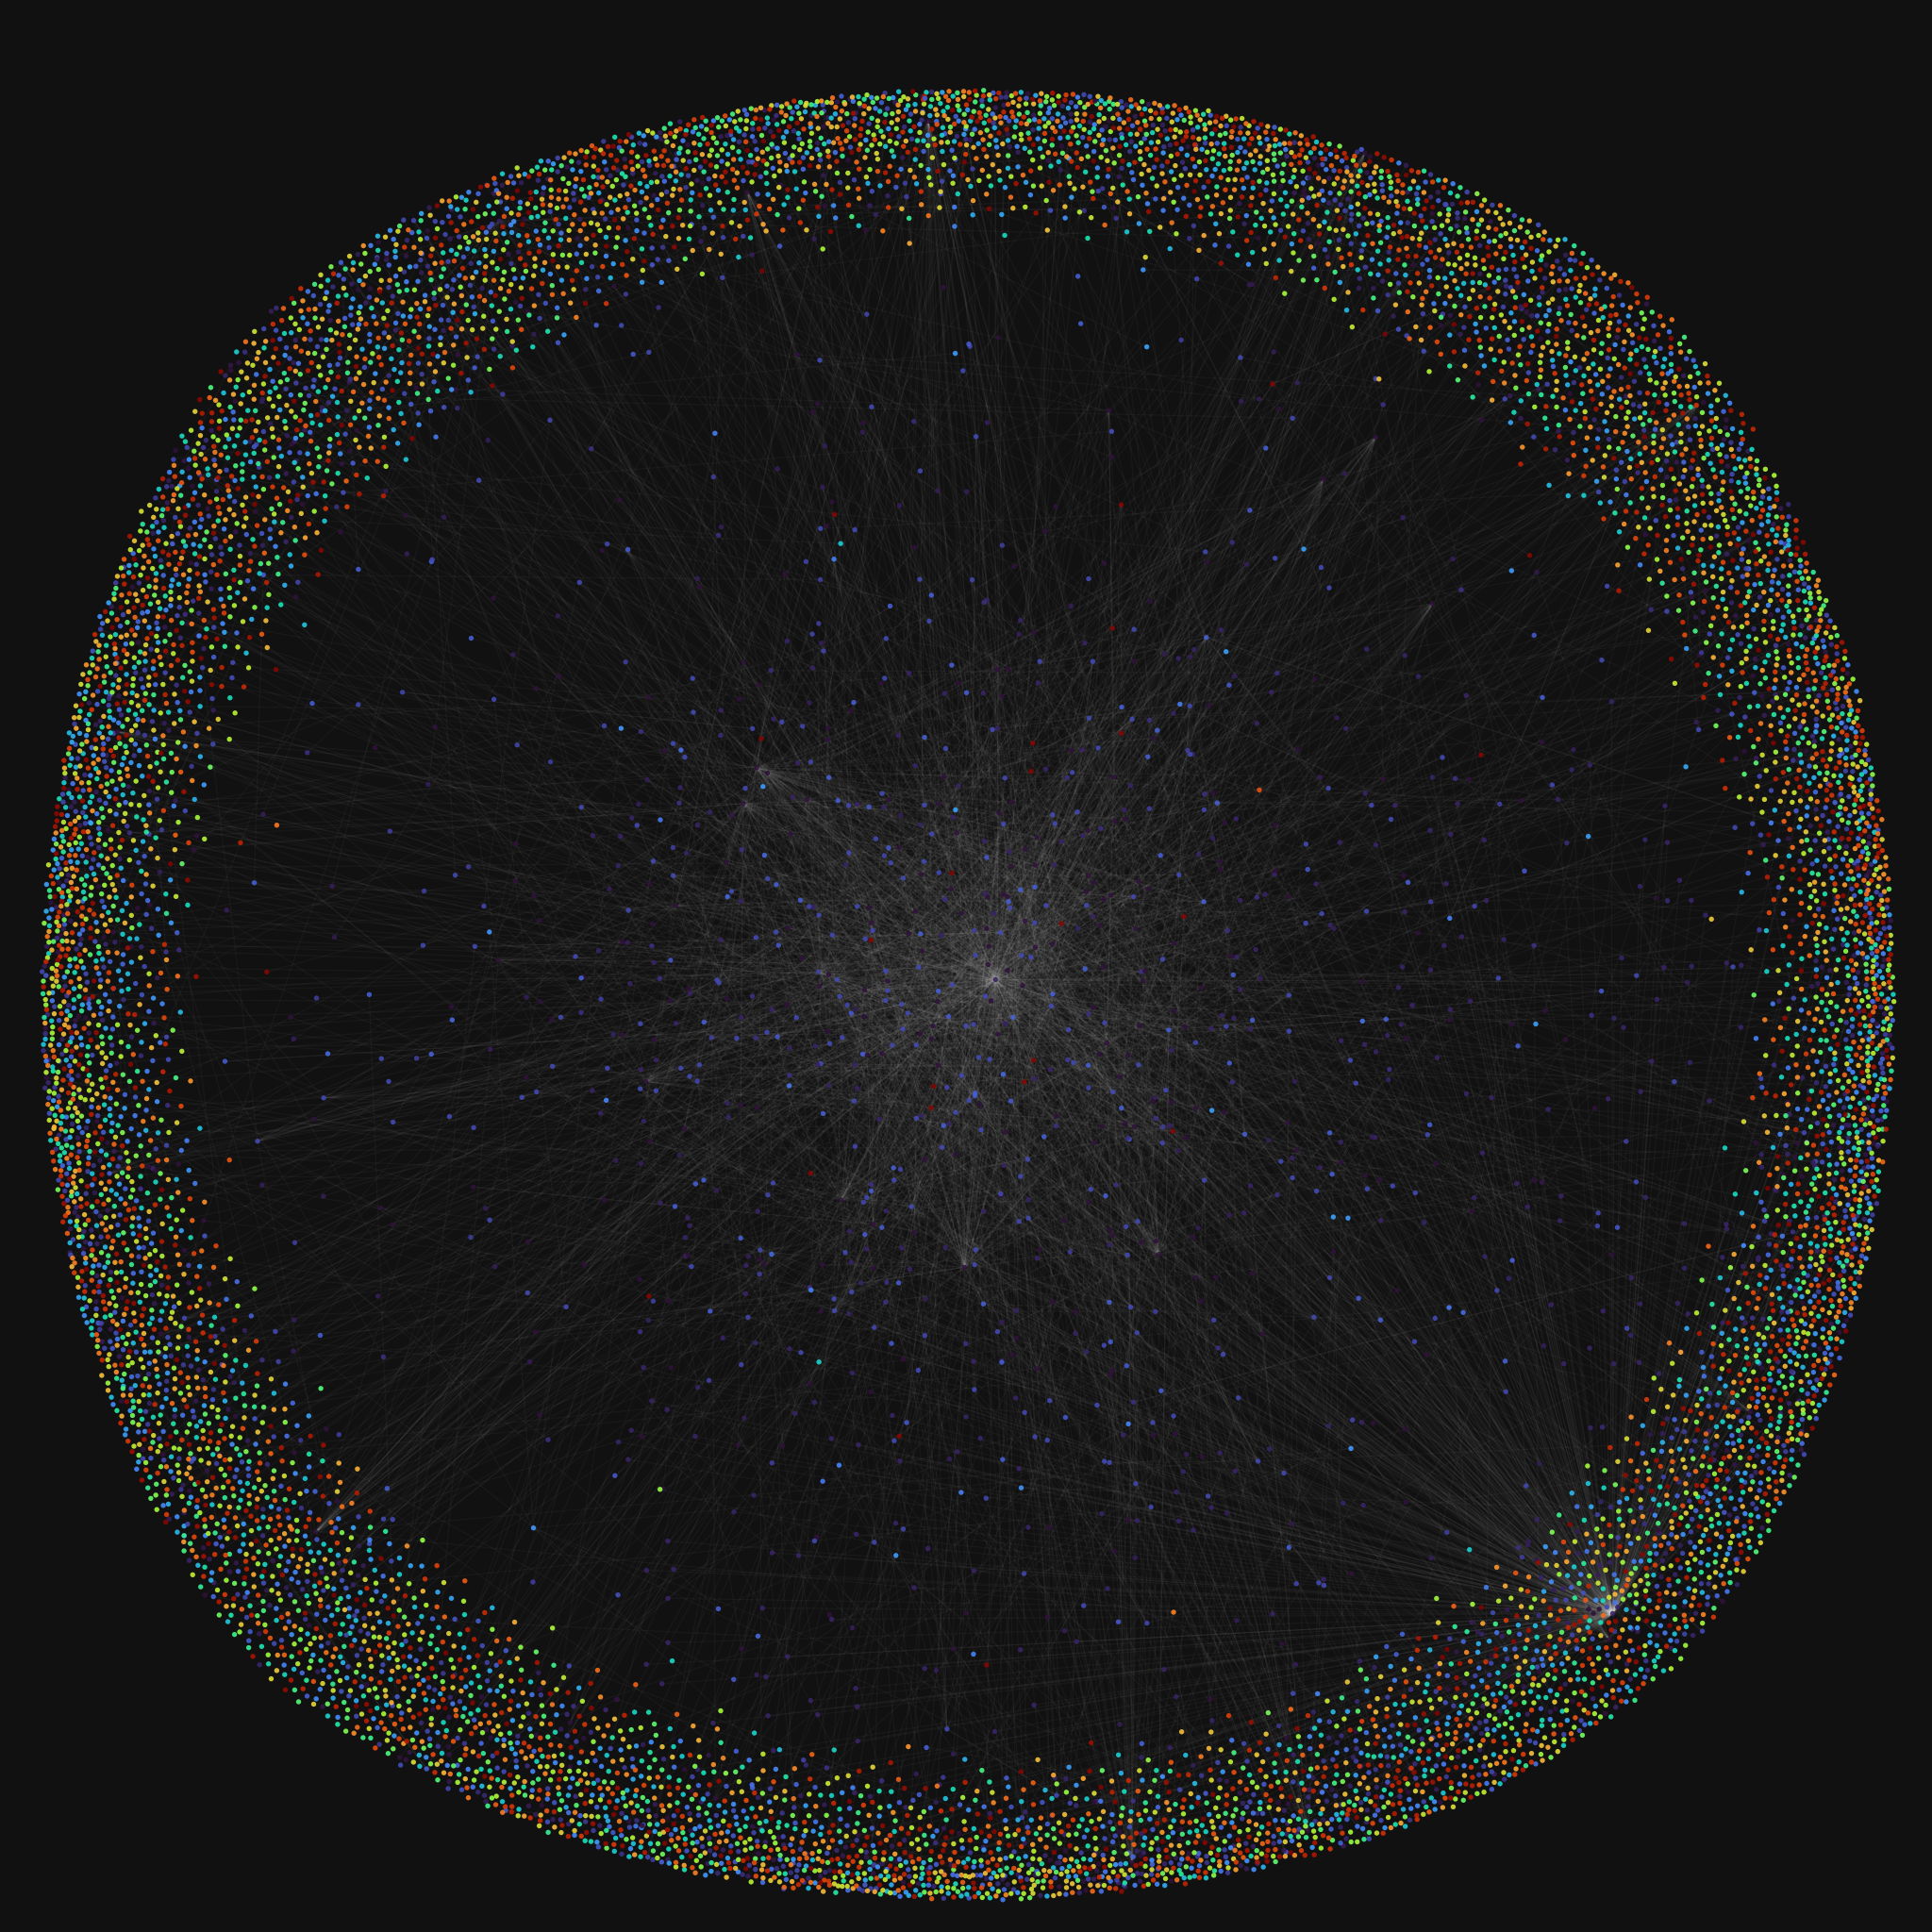
\includegraphics[width=0.8\textwidth]{./figures/rede_completa.png}
    \caption{Visualização global da rede de influências artísticas original. A disposição em nuvem evidencia a altíssima esparsidade estrutural ($D \approx 0.000027$) e a fragmentação inerente do sistema em múltiplas "ilhas" ou bacias menores isoladas temporariamente e geograficamente da rede principal.}
    \label{fig:rede_geral}
\end{figure}

\section{Caracterização Topológica da Rede}

A distribuição de conectividade dita a resiliência e a dinâmica de propagação de um grafo. Redes de influência cultural frequentemente assumem uma topologia Livre de Escala (\textit{Scale-Free}), onde a distribuição da probabilidade de grau decai segundo uma lei de potência ($P(k) \sim k^{-\gamma}$).

Para validar esta hipótese, utilizou-se a Estimativa de Máxima Verossimilhança (MLE) via biblioteca \texttt{powerlaw}. A estimativa inicial para o grau de saída apontou um expoente $\gamma \approx 2.27$. No entanto, o teste de robustez via \textit{Loglikelihood Ratio} ($R = -6.8966$, $p$-valor $= 5.32 \times 10^{-12}$) demonstrou que uma distribuição Lognormal ajusta-se de forma estatisticamente superior aos dados empíricos em comparação à Lei de Potência pura. Ainda que a distribuição seja Lognormal, a presença de uma cauda pesada, evidenciada visualmente na Figura \ref{fig:dist_grau}, confirma a existência de "\textit{hubs}" super-espalhadores de tendências artísticas.

\begin{figure}[htpb]
    \centering
    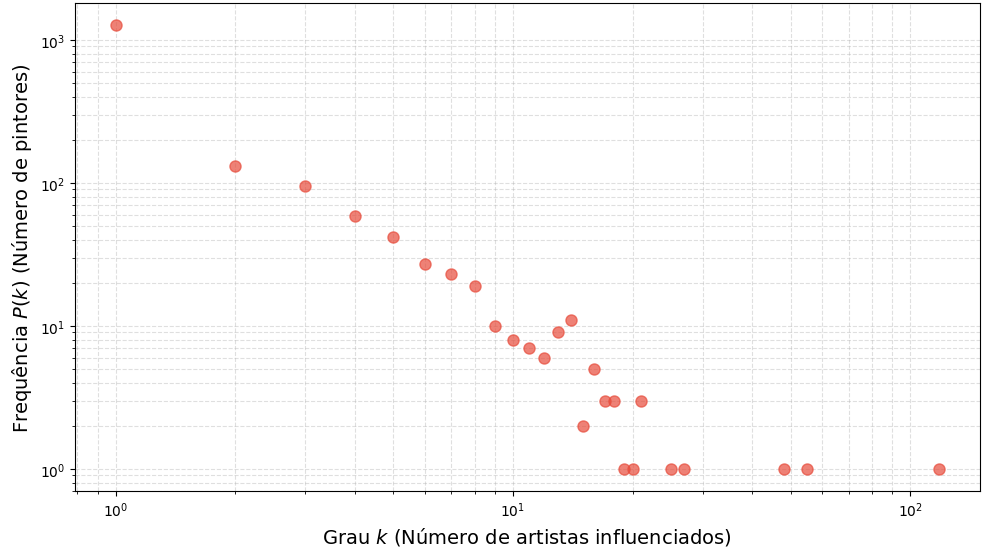
\includegraphics[width=0.8\textwidth]{./figures/dist_grau.png}
    \caption{Distribuição empírica do grau de saída (\textit{Out-Degree}) em escala \textit{log-log}. O decaimento em cauda pesada ilustra a topologia fortemente assimétrica da rede: a imensa maioria dos artistas exerce pouca influência direta, enquanto uma seleta minoria (\textit{hubs}) irradia tendências para uma grande parcela do sistema.}
    \label{fig:dist_grau}
\end{figure}

\subsection{Métricas de Centralidade e Influência}

Para quantificar a importância individual de cada pintor, quatro métricas topológicas fundamentais foram computadas:
\begin{itemize}
    \item \textbf{Grau de Entrada (\textit{In-Degree}):} Mede a suscetibilidade do nó. Altos valores indicam pintores que absorveram técnicas de múltiplas fontes.
    \item \textbf{Grau de Saída (\textit{Out-Degree}):} Mede o alcance direto. \textit{Hubs} neste critério são grandes difusores de tendências.
    \item \textbf{\textit{PageRank}:} Diferentemente do grau, o \textit{PageRank} não avalia apenas a quantidade, mas a qualidade das conexões. Um artista pontua alto se influenciou outros nomes canônicos da rede.
    \item \textbf{Intermediação (\textit{Betweenness}):} Identifica pontes. Artistas com alta intermediação são gargalos por onde um estilo transita entre gerações ou comunidades distintas.
\end{itemize}

A Tabela \ref{tab:centralidades} ilustra o comportamento destas métricas para artistas selecionados e demonstra o fenômeno dos nós ruidosos na prática. Isaac Levitan demonstra altíssima centralidade em todos os quesitos, atuando tanto como um grande absorvedor (\textit{In-Degree} 156) quanto como um pilar canônico (\textit{PageRank} de 0.0093). Em paralelo, artefatos do \textit{dataset} como \textit{male-portraits} alcançam graus de saída superiores aos de muitos pintores reais, comprovando como características amplas de gênero artístico agem topologicamente como \textit{hubs} de difusão de tendências, influenciando dezenas de nós subsequentes.

\begin{table}[htpb]
    \centering
    \caption{Métricas de centralidade computadas para uma amostra de vértices reais e artefatos semânticos do \textit{dataset}.}
    \label{tab:centralidades}
    \begin{tabular}{@{}lcccc@{}}
        \toprule
        \textbf{Nó / Vértice}    & \textbf{In-Degree} & \textbf{Out-Degree} & \textbf{PageRank} & \textbf{Betweenness} \\ \midrule
        Isaac Levitan            & 156                & 118                 & 0.00932           & 0.00125              \\
        Alexander Ivanov         & 1                  & 55                  & 0.00011           & 0.00084              \\
        Umberto Boccioni         & 4                  & 48                  & 0.00027           & 0.00037              \\
        male-portraits (ruído)   & 4                  & 27                  & 0.00013           & 0.00026              \\
        female-portraits (ruído) & 3                  & 25                  & 0.00013           & 0.00015              \\ \bottomrule
    \end{tabular}
\end{table}

\subsection{Transitividade e Assortatividade}

A transitividade global da rede é excepcionalmente baixa (0.0075), e o coeficiente de aglomeração médio resulta em 0.0021. No contexto histórico, isso indica que "triângulos" fechados de influência (onde três pintores se influenciam mutuamente) são raros.

Essa característica é complementada pelo Coeficiente de Assortatividade negativo ($-0.1973$). Uma rede desassortativa revela um comportamento estritamente hierárquico na transmissão do conhecimento: grandes mestres (\textit{hubs} de altíssimo grau) tendem a influenciar majoritariamente uma massa de aprendizes de baixo grau.

\section{Componente Gigante e Comunidades}

Devido à vasta extensão espaço-temporal da história da arte, a rede original fragmenta-se em diversas ilhas de conexões isoladas. Para viabilizar a análise de fluxo de informação e as simulações epidêmicas, extraiu-se o Maior Componente Fracamente Conectado (\textit{Weakly Connected Giant Component}). Este componente concentra 1.583 nós (13,2\% da rede original) e 3.234 arestas.

A topologia deste núcleo exibe propriedades clássicas de "Pequeno Mundo" (\textit{Small-World}). O diâmetro máximo encontrado foi de 11 saltos, com um caminho mais curto médio de 4,88. Isso sugere que, apesar das barreiras de época, qualquer inovação estética desenvolvida na história da arte europeia poderia alcançar qualquer outro pintor na rede principal em menos de 5 "graus de separação".

\subsection{Detecção de Comunidades e a Descentralização dos Movimentos}

O algoritmo de \textit{Louvain} foi aplicado para otimizar a modularidade do grafo, atingindo um valor expressivo de $Q = 0.7274$. Este índice indica uma estrutura comunitária forte, onde as influências ocorrem primariamente de forma intragrupo, caracterizando a coesão local de ateliês ou escolas artísticas ("panelinhas"). A Figura \ref{fig:comunidades_louvain} ilustra espacialmente a segregação topológica e a densidade destas partições dentro do Componente Gigante.

Um resultado notável desta etapa é a identificação matemática da fragmentação de movimentos artísticos reais. Comunidades estruturalmente independentes apresentaram rótulos predominantes idênticos, como o \textit{Art Nouveau} e o Barroco.

Como o método de \textit{Louvain} opera estritamente sobre a densidade topológica das arestas (sendo cego aos atributos semânticos dos vértices), esta fragmentação não constitui um erro de clusterização, mas uma descoberta analítica sobre a descentralização do contágio artístico. O Barroco, por exemplo, bifurca-se topologicamente entre as tradições Católica e Protestante. Esses grupos se desenvolveram simultaneamente sob o mesmo rótulo estilístico, porém isolados por barreiras geográficas e religiosas, resultando em bacias de influência topologicamente separadas.

\begin{figure}[htpb]
    \centering
    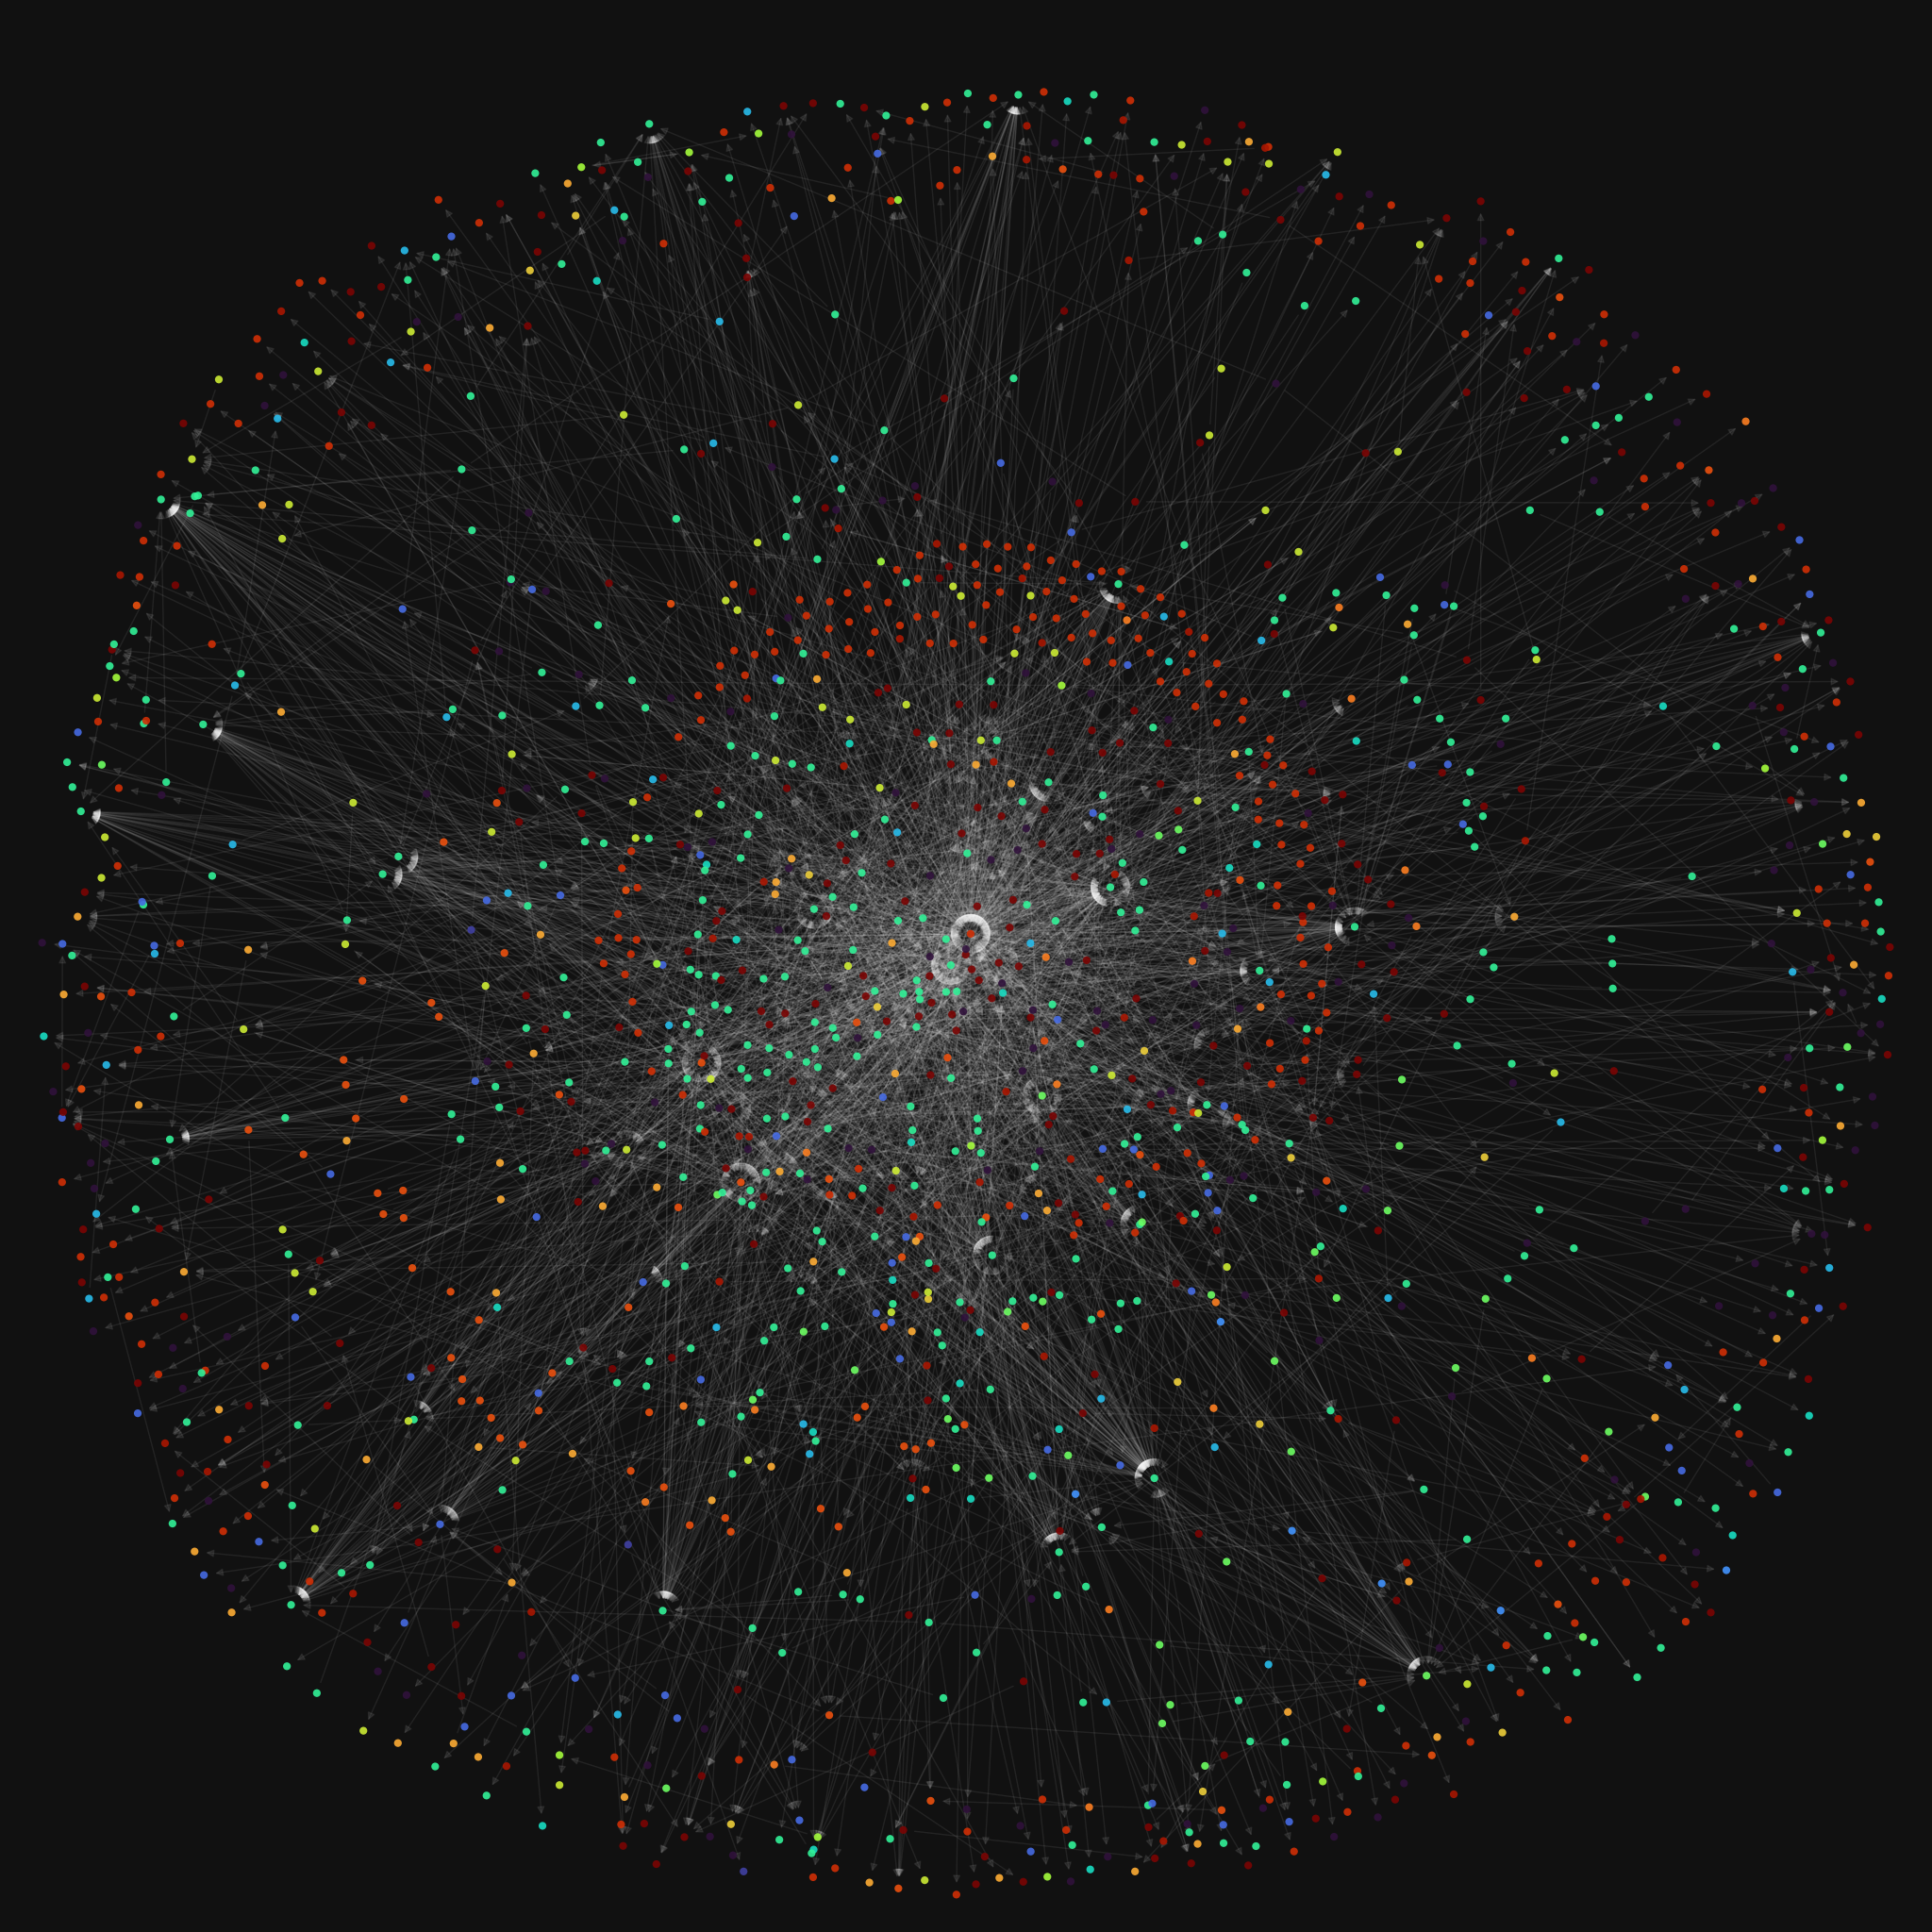
\includegraphics[width=0.9\textwidth]{./figures/g_gigante-comunidades.png}
    \caption{Grafo direcionado do Componente Gigante colorido pelas partições detectadas pelo algoritmo de Louvain. A visualização atesta a alta modularidade da rede ($Q = 0.7274$), evidenciando grupos fortemente conectados internamente ("escolas artísticas"), mas limitados por fronteiras esparsas na conexão com grupos paralelos.}
    \label{fig:comunidades_louvain}
\end{figure}

\section{Processos Dinâmicos de Influência}

A difusão de inovações estéticas pode ser tratada matematicamente como um processo epidêmico. Tradicionalmente, modelos compartimentais assumem populações perfeitamente misturadas (aproximação de campo médio). No contexto deste trabalho, essa premissa é descartada: a dinâmica torna-se um processo estocástico de tempo discreto, estritamente governado pela matriz de adjacência $A_{ij}$ da rede \cite{ndlib_ref}.

\subsection{O Modelo SIR e a Seta do Tempo}

O modelo SIR (Suscetível-Infectado-Removido) clássico, em sua formulação contínua, é descrito pelo seguinte sistema de equações diferenciais ordinárias:
\begin{align}
    \frac{dS}{dt} & = -\beta \frac{S I}{N}           \\
    \frac{dI}{dt} & = \beta \frac{S I}{N} - \gamma I \\
    \frac{dR}{dt} & = \gamma I
\end{align}

Na topologia de rede, a probabilidade de um pintor suscetível $i$ adotar a nova vanguarda no tempo $t$ é dada por $P(S_i \to I_i) = 1 - (1 - \beta)^{m_i}$, onde $m_i$ é o número de vizinhos diretos infectados, e $\beta = 0.15$ é a taxa de contágio empírica. A recuperação (abandono do estilo) ocorre com probabilidade $\gamma = 0.05$.

Para simular o contágio ao longo de toda a história sem violar a cronologia (nós recentes influenciando nós antigos por ruídos ou influências póstumas), o Componente Gigante foi forçado a se tornar um Grafo Direcionado Acíclico (DAG). A remoção de 3.029 arestas que violavam a "seta do tempo" permitiu que a simulação representasse estritamente as sucessivas gerações de influência.

Adicionalmente, elaborou-se um recorte temporal (1850 a 1920, contendo 236 nós e 433 arestas) para simular o contágio iterativo em um grupo de pintores que de fato coexistiram, permitindo a observação visual da difusão em tempo real.

\begin{figure}[htpb]
    \centering
    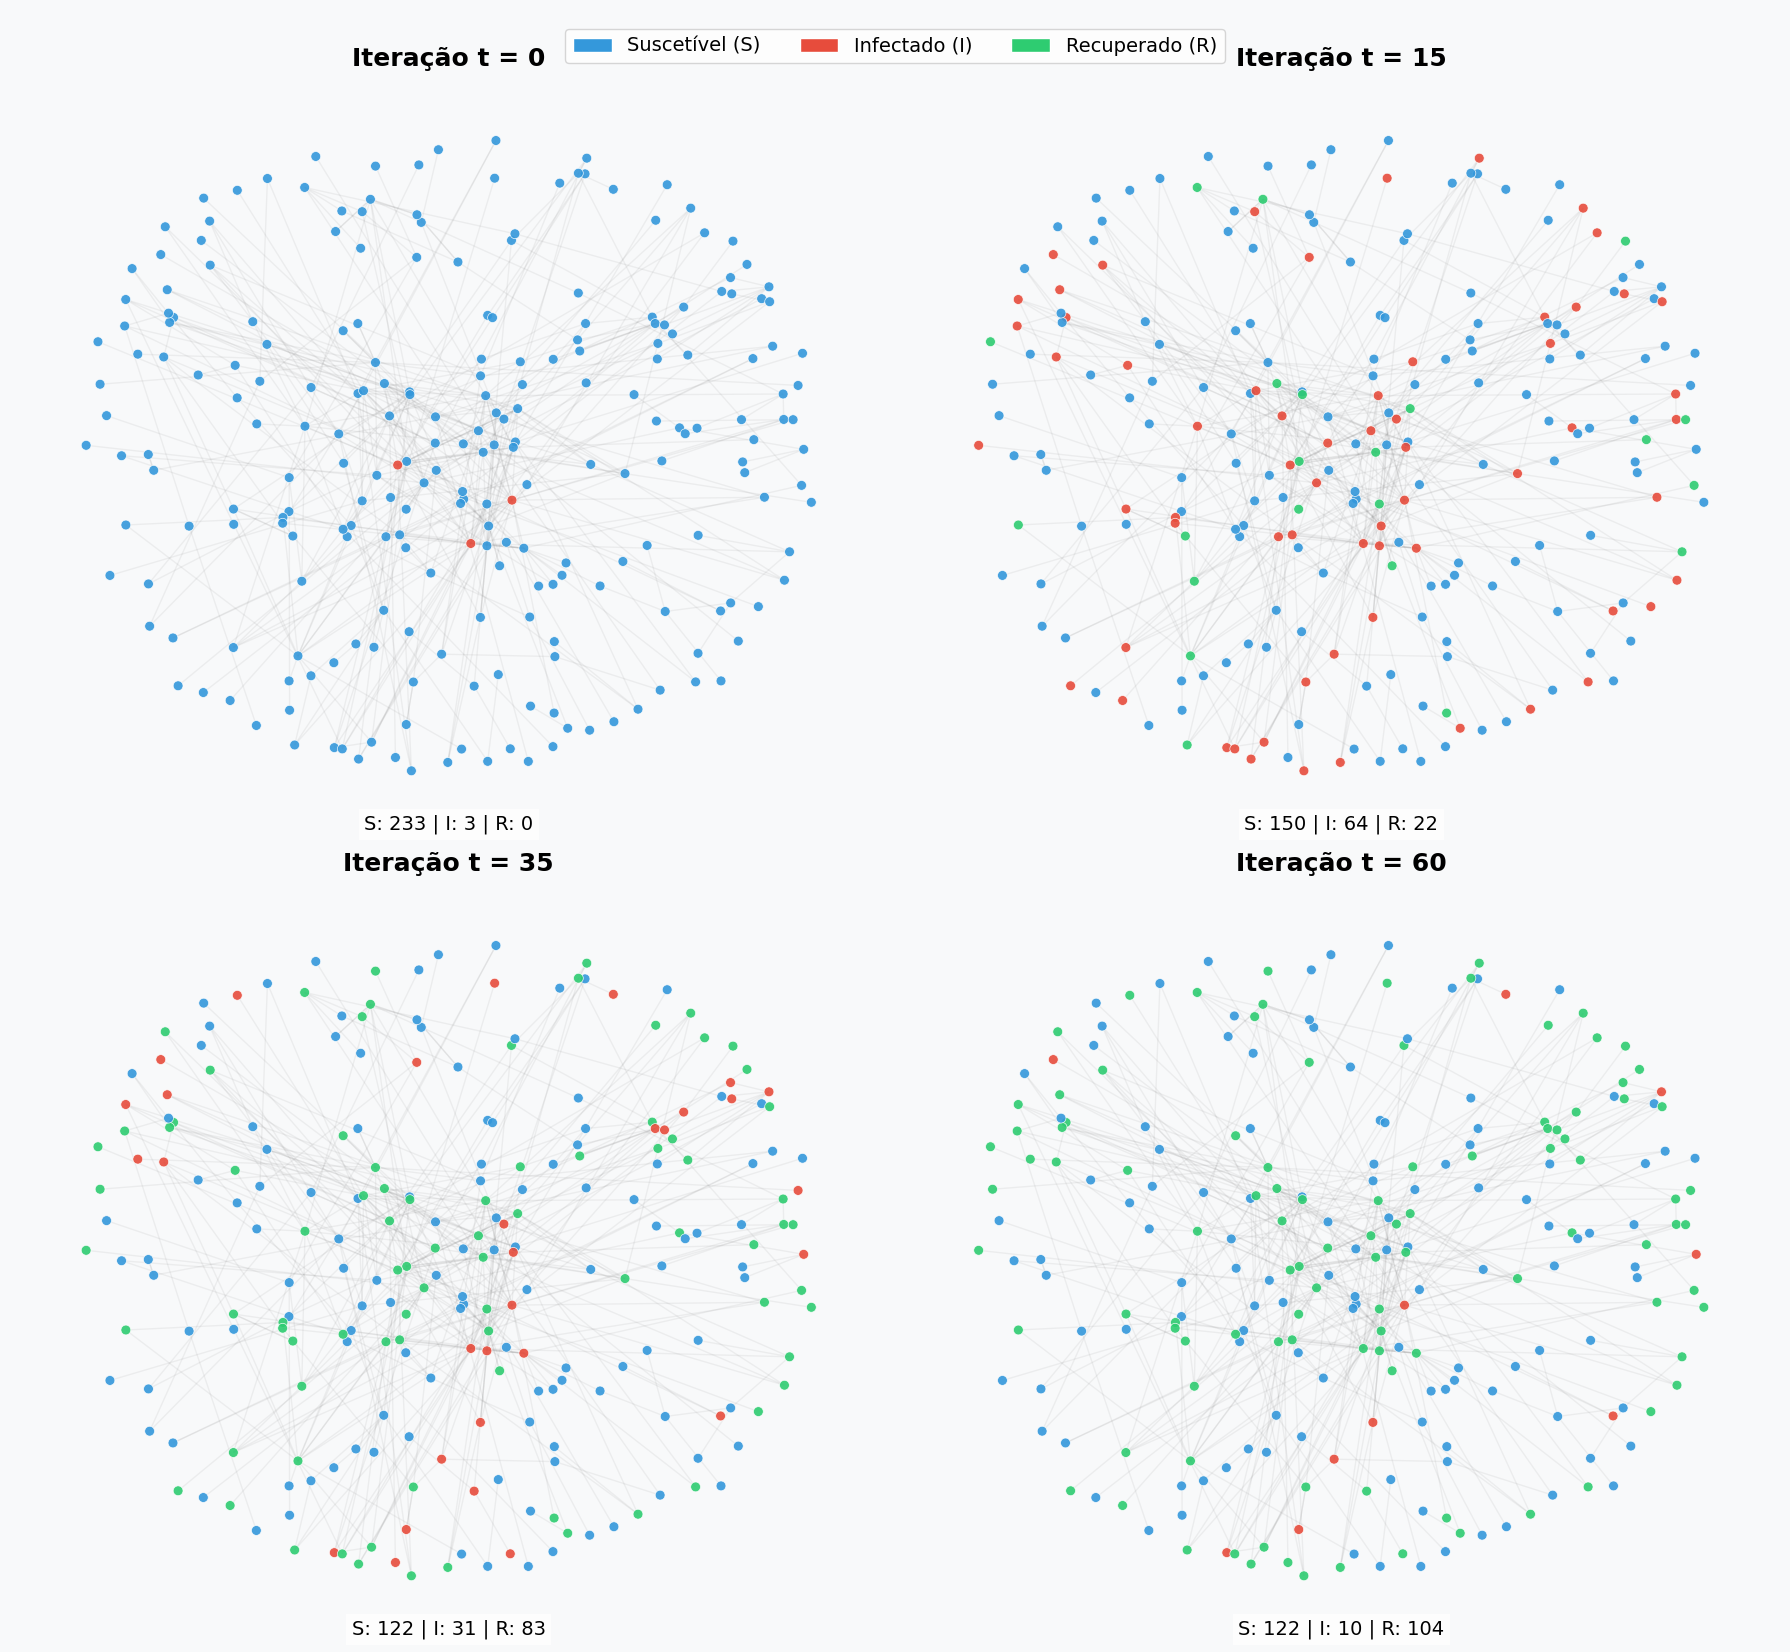
\includegraphics[width=0.9\textwidth]{./figures/sir_simulacao.png}
    \caption{Simulação do Modelo SIR: Propagação do estilo artístico ao longo de 60 iterações no recorte temporal de 1850-1920.}
    \label{fig:sir_simulacao}
\end{figure}

\subsection{Dinâmica Cíclica e Latência: O Modelo SEIS}

Uma limitação do modelo SIR clássico, quando aplicado a fenômenos socioculturais, é a premissa da imunidade permanente (o estado $R$). Na história da arte, artistas frequentemente possuem "fases" e podem revisitar estilos do passado ou abandonar uma vanguarda para voltar a ser influenciados por outras tendências. Para capturar essa dinâmica cíclica, somada ao tempo inerente de assimilação de uma técnica, aplicamos o modelo SEIS (Suscetível-Exposto-Infectado-Suscetível).

Sob a aproximação clássica de campo médio para populações homogêneas, a dinâmica contínua do modelo é descrita pelo seguinte sistema de equações diferenciais ordinárias:
\begin{align}
    \frac{dS}{dt} & = -\beta \frac{S I}{N} + \lambda I \\
    \frac{dE}{dt} & = \beta \frac{S I}{N} - \alpha E   \\
    \frac{dI}{dt} & = \alpha E - \lambda I
\end{align}

No entanto, em uma abordagem estruturada por redes complexas, o processo se torna estocástico e de tempo discreto, sendo estritamente condicionado à vizinhança topológica de cada pintor. As transições de estado para cada nó $i$ no instante $t$ obedecem às seguintes probabilidades e regras analíticas:

\begin{itemize}
    \item \textbf{$S \to E$ (Suscetível para Exposto):} Ocorre por meio do contágio direcional. A probabilidade de um nó suscetível $i$ ser exposto e entrar na fase de latência é formulada por $P(S_i \to E_i) = 1 - (1 - \beta)^{m_i}$, onde $m_i$ representa o número de vizinhos diretos (influenciadores) de $i$ que estão no estado Infectado ($I$) no tempo $t$.
    \item \textbf{$E \to I$ (Exposto para Infectado):} O término do período latente — que representa empiricamente o intervalo de estudo e assimilação da nova técnica — ocorre de forma espontânea com uma probabilidade constante por unidade de tempo definida por $P(E_i \to I_i) = \alpha$.
    \item \textbf{$I \to S$ (Infectado para Suscetível):} Representa a "mudança de fase" do artista. O abandono temporal do estilo e o consequente retorno ao estado de suscetibilidade (aberto a novas inspirações) ocorre com probabilidade constante $P(I_i \to S_i) = \lambda$.
\end{itemize}

A Figura \ref{fig:seis_simulacao} ilustra a propagação iterativa sob este modelo ao longo de 200 iterações. Em contraste direto com o esgotamento natural observado no modelo SIR, a simulação do SEIS evidencia a sustentação de uma dinâmica de ativação cíclica. Este comportamento demonstra uma aderência metodológica substancialmente superior à realidade fluida, retrospectiva e não-definitiva da produção artística.

\begin{figure}[htpb]
    \centering
    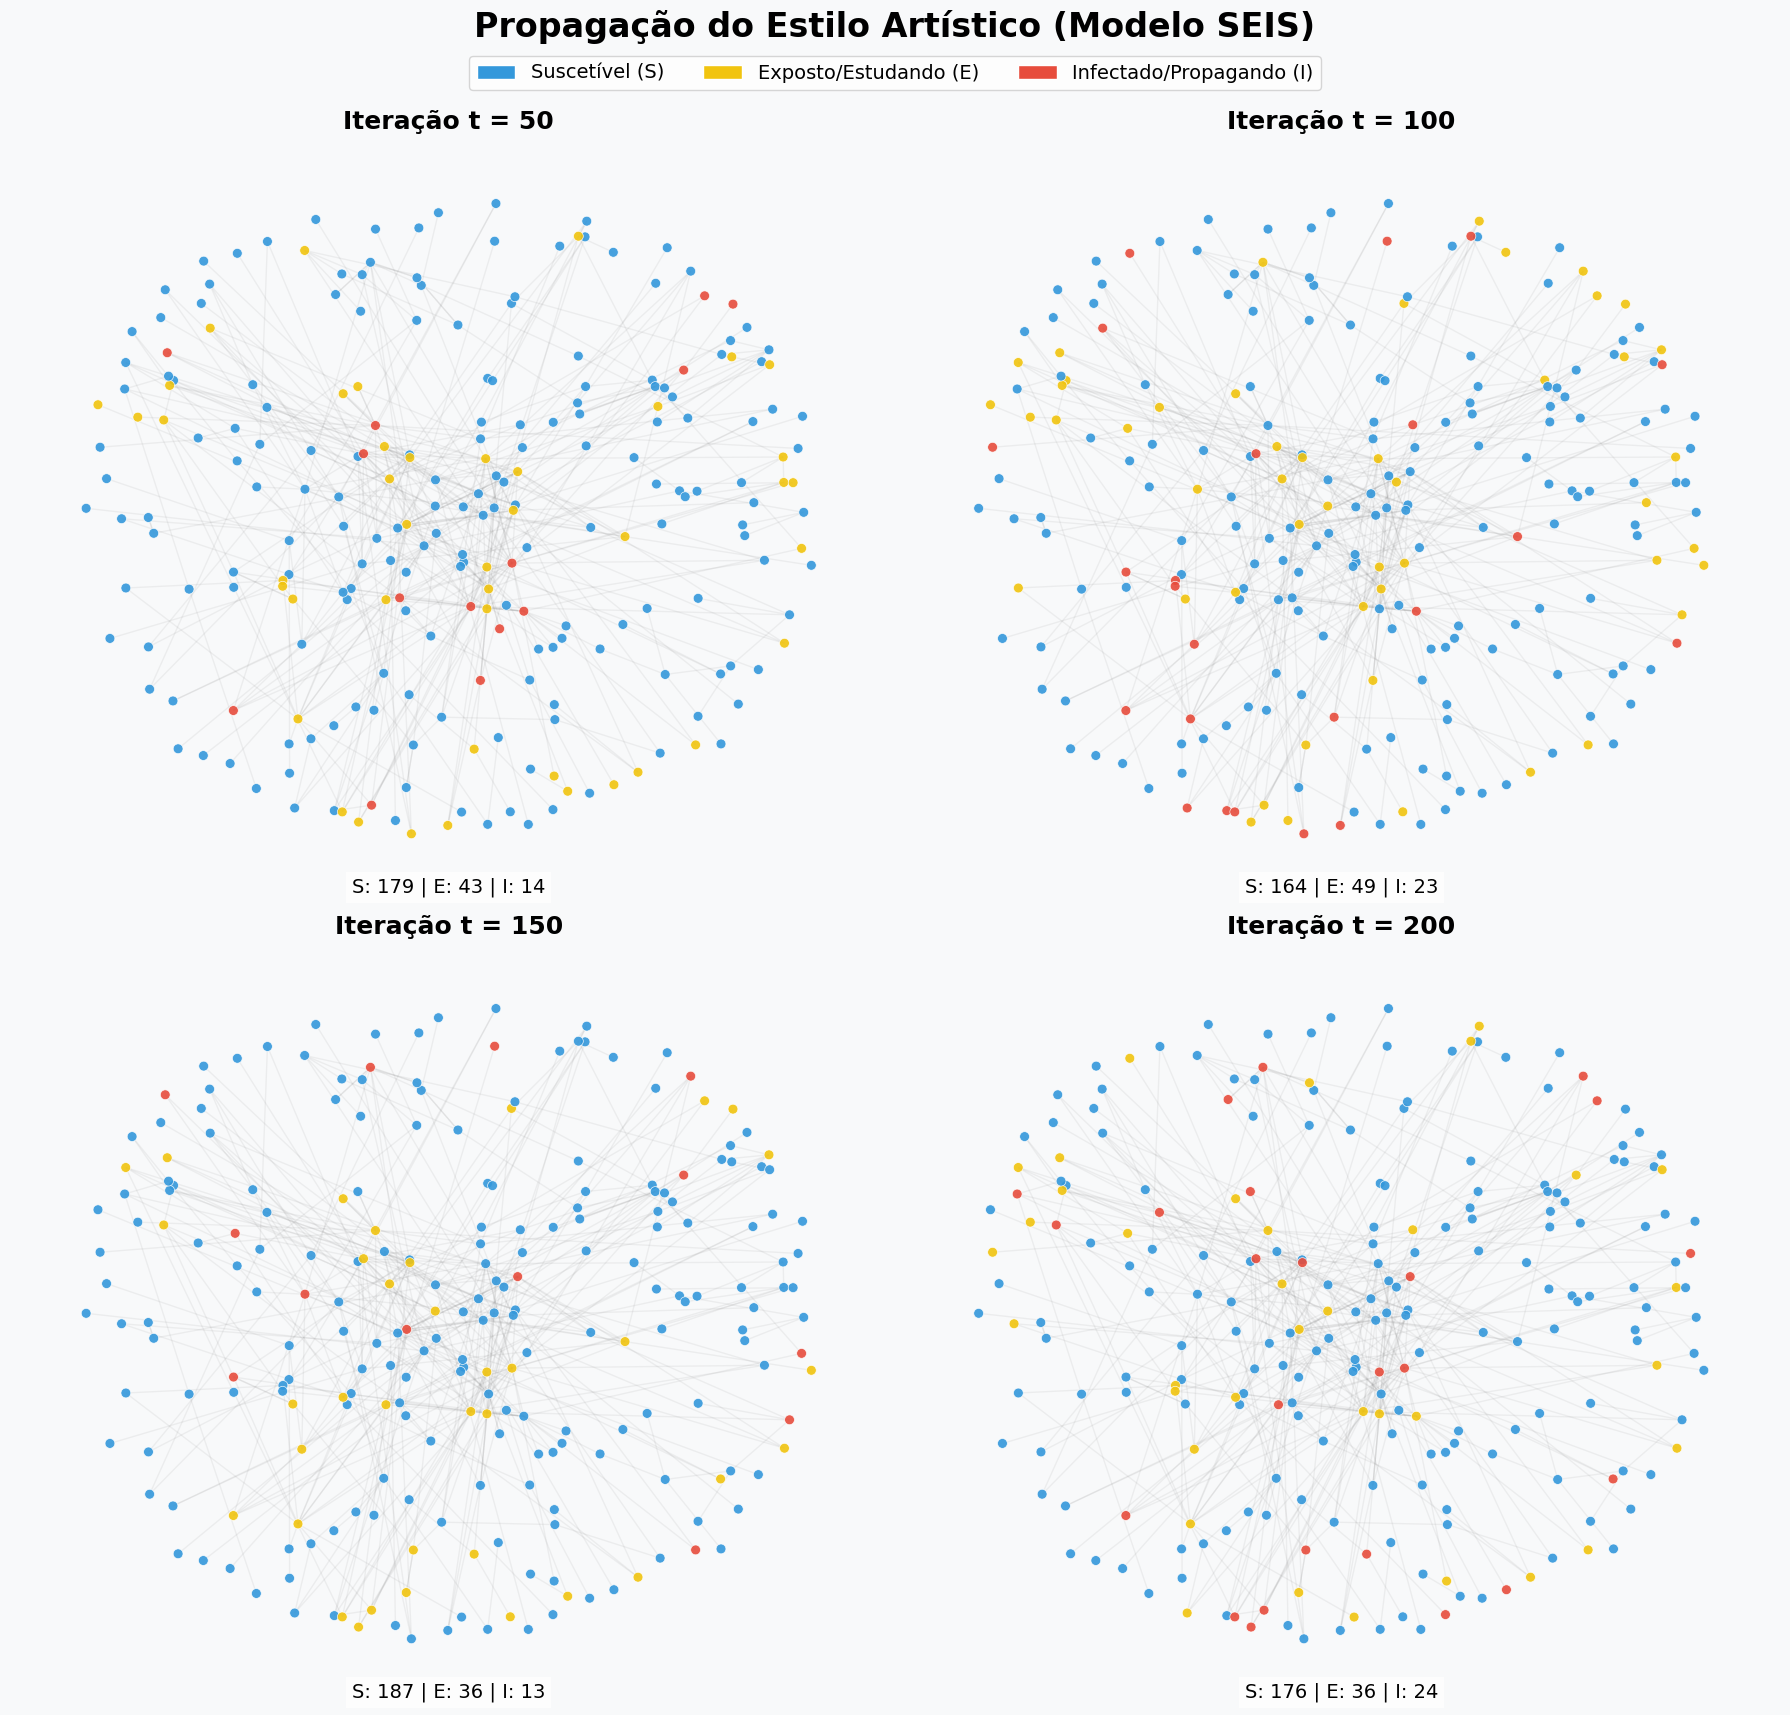
\includegraphics[width=0.9\textwidth]{./figures/seis_simulacao.png}
    \caption{Simulação do Modelo SEIS: Evolução da dinâmica cíclica e do período de latência na arte ao longo de 200 iterações no recorte temporal da rede (1850-1920).}
    \label{fig:seis_simulacao}
\end{figure}

\section{Validação Estatística com Modelos Nulos}

Para atestar que as propriedades estruturais observadas (alta aglomeração e distâncias curtas) possuem significado sociológico e não são fruto do acaso, a rede real foi comparada a três modelos nulos (Tabela \ref{tab:modelos_nulos}) gerados sobre o componente gigante não-direcionado \cite{barabasi_network_science, newman_networks}.

\begin{table}[htpb]
    \centering
    \caption{Comparação de métricas globais entre a rede real de arte e os modelos nulos.}
    \label{tab:modelos_nulos}
    \begin{tabular}{@{}lcccc@{}}
        \toprule
        \textbf{Métrica}    & \textbf{Rede Real} & \textbf{Erdős-Rényi} & \textbf{Configuração} & \textbf{Barabási-Albert} \\ \midrule
        Caminho Médio ($L$) & 4.8867             & 5.4374               & 3.9646                & 4.2820                   \\
        Aglomeração ($C$)   & 0.0300             & 0.0035               & 0.0278                & 0.0190                   \\ \bottomrule
    \end{tabular}
\end{table}

A análise comparativa, corroborada pela projeção espacial dos grafos ilustrada na Figura \ref{fig:modelos_nulos}, permite classificar a rede de influências da arte sob dois prismas fundamentais:

\begin{enumerate}
    \item \textbf{Rede de Pequeno Mundo (\textit{Small-World}):} O coeficiente de aglomeração da rede real ($C = 0.0300$) é quase dez vezes superior ao esperado por uma distribuição puramente aleatória via Erdős-Rényi ($C_{ER} = 0.0035$). Simultaneamente, o caminho mais curto ($L = 4.8867$) mantém-se diminuto, inclusive inferior ao limite aleatório. Isso comprova estatisticamente a forte coesão local (as "escolas" artísticas) combinada a uma rápida capacidade de transmissão global.

    \item \textbf{Dinâmica de Apego Preferencial:} A topologia real converge expressivamente para os modelos de Configuração e Barabási-Albert (BA). A aproximação com as métricas do modelo BA ($L_{BA} = 4.2820$, $C_{BA} = 0.0190$) valida que o mecanismo subjacente à história da arte é o apego preferencial ("o rico fica mais rico"). A influência não se distribui ao acaso; ela concentra-se em grandes mestres cujo peso histórico atrai desproporcionalmente as conexões (atenção e estudo) de novas gerações de aprendizes. Essa convergência é visualmente notória na Figura \ref{fig:modelos_nulos}, onde a rede real e o modelo BA exibem a mesma assinatura topológica: núcleos densos concentrados em poucos super-espalhadores, em forte contraste com a malha dispersa e homogênea do modelo aleatório.
\end{enumerate}

\begin{figure}[htpb]
    \centering
    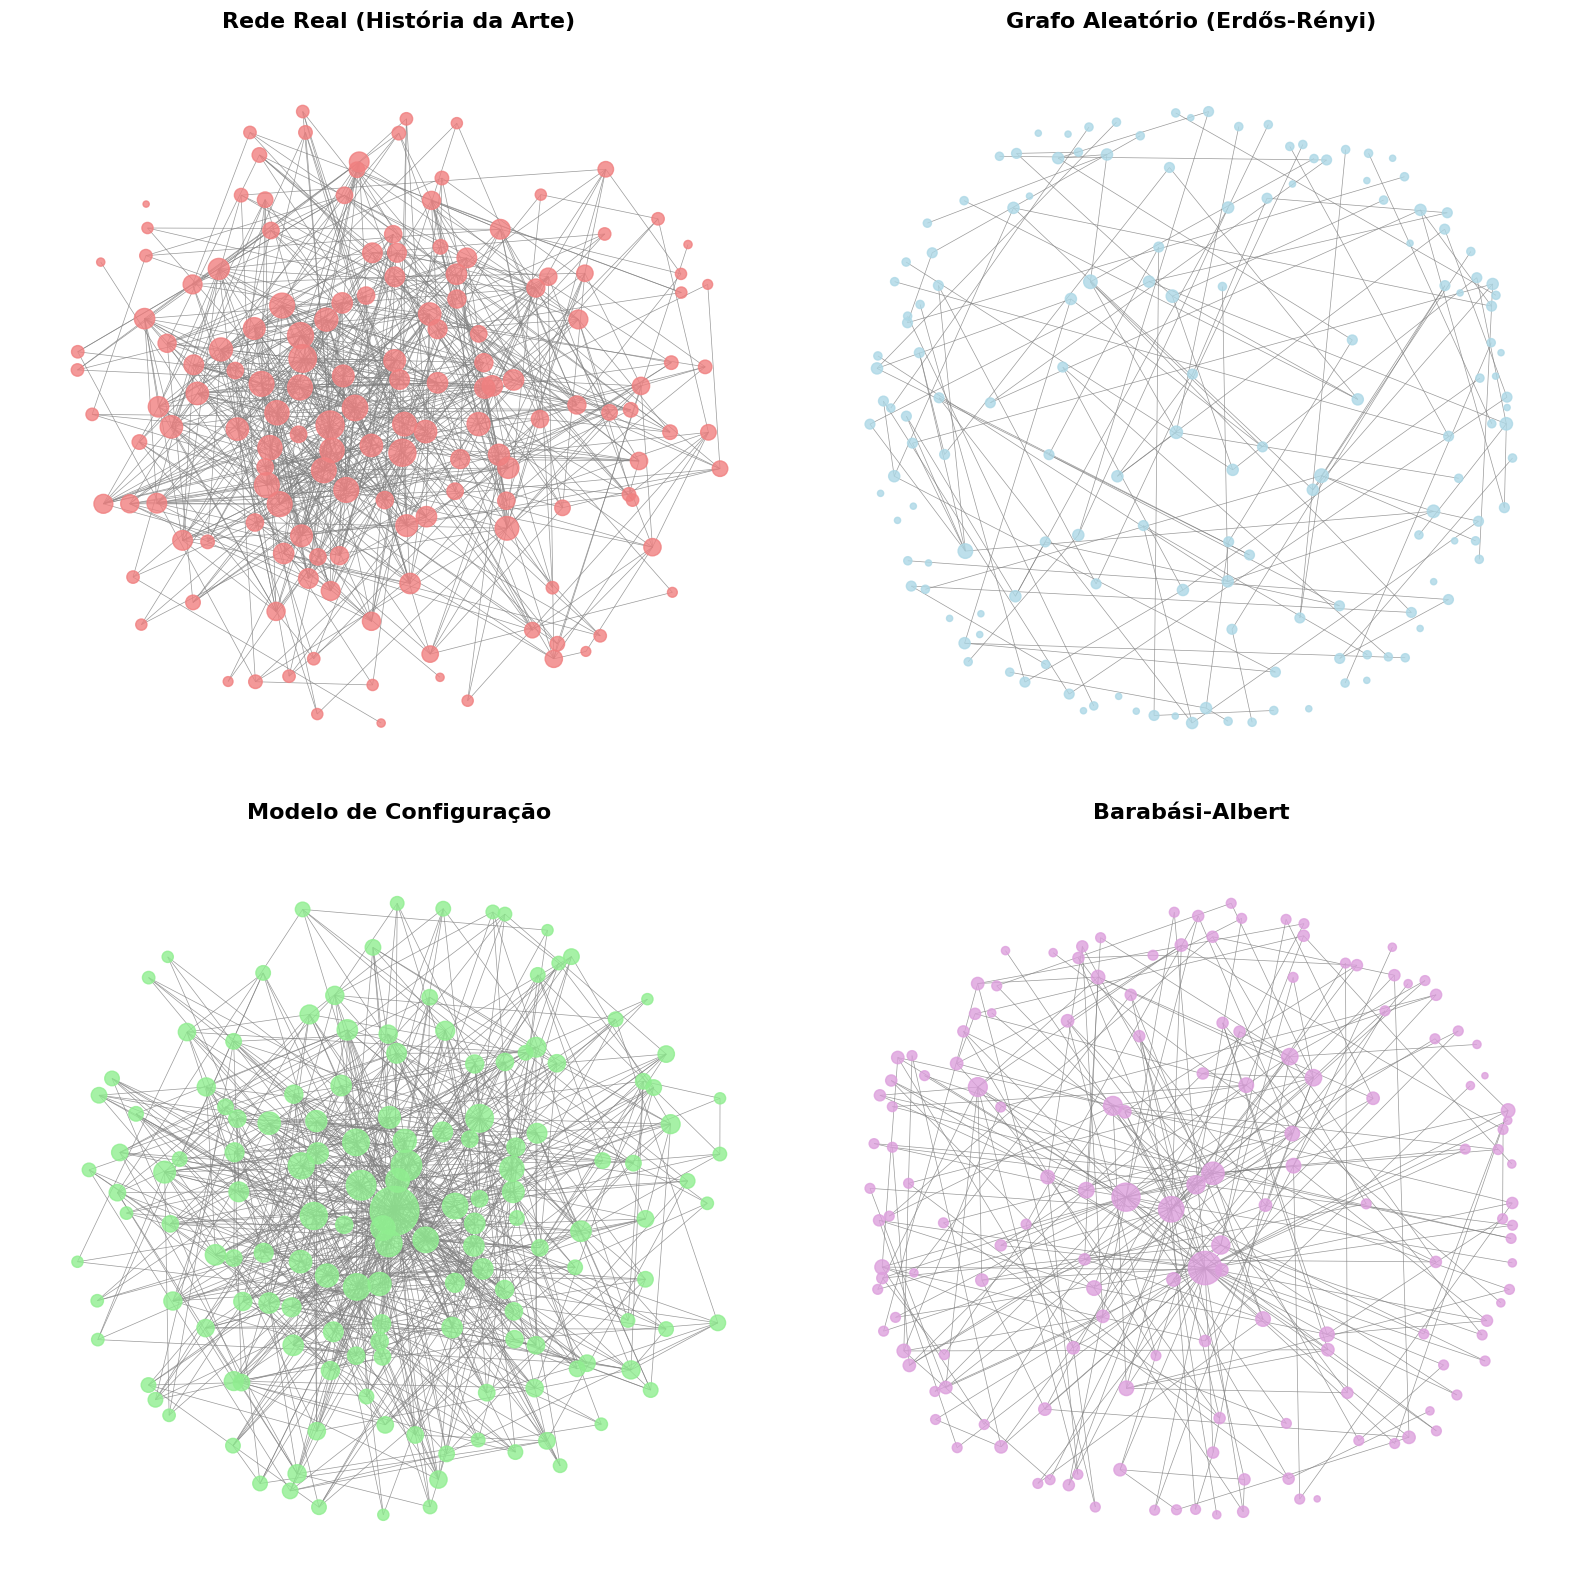
\includegraphics[width=\textwidth]{./figures/modelos_nulos.png}
    \caption{Comparação topológica visual entre um subgrafo representativo da rede real de arte e as topologias sintéticas equivalentes geradas pelos modelos nulos. O dimensionamento dos vértices é proporcional ao seu respectivo grau. A representação evidencia a falha do modelo de Erdős-Rényi em capturar a heterogeneidade do sistema, contrastando com o notável alinhamento estrutural entre a rede real e o modelo de Barabási-Albert na formação de \textit{hubs} centrais.}
    \label{fig:modelos_nulos}
\end{figure}

\section{Conclusão}

A modelagem da história da arte como uma rede complexa demonstrou que a evolução estética transcende a cronologia linear, comportando-se matematicamente como um processo de difusão de conhecimento governado por regras topológicas definidas. A análise estrutural confirmou que o fluxo de influências opera sob uma dinâmica de apego preferencial. A validação contra o modelo de Barabási-Albert justifica a topologia hierárquica e desassortativa do sistema: uma minoria de grandes mestres atrai de forma assimétrica a atenção das novas gerações, atuando como super-espalhadores de conhecimento.

Além disso, a abstração matemática foi capaz de redescobrir fenômenos histórico-geográficos de forma cega. A detecção de comunidades otimizou a rede e mapeou a descentralização de movimentos como o Barroco, isolando vertentes desenvolvidas paralelamente, porém separadas por barreiras religiosas e espaciais.

No âmbito dos processos dinâmicos, a simulação estocástica revelou que epidemias culturais são descritas com maior precisão metodológica pelo modelo SEIS do que pelo clássico SIR. A adoção de um período de latência e a remoção da premissa de imunidade permanente capturam de forma mais realista o tempo necessário para a assimilação de uma técnica e a fluidez intrínseca às fases da carreira de um pintor. Em suma, os resultados obtidos validam quantitativamente a hipótese de que a sucessão de vanguardas na arte obedece a propriedades estruturais mensuráveis, oferecendo uma integração robusta entre a ciência de redes e a sociologia cultural.

\renewcommand{\refname}{Referências}
\bibliographystyle{unsrt}
\bibliography{referencias}


\end{document}